\section{Simple Harmonic Motion}

object moves back and forth about an equilibrium position $\longrightarrow$ oscillatory motion

must have restoring force always pointing towards equilibrium position

acceleration is in opposite direction to displacement

if magnitude of acceleration is proportional to displacement $\longrightarrow$ simple harmonics

defining equation for simple harmonic oscillation: $\boxed{a=-\omega^2x}$ or $\boxed{\dddt{x} = -\omega^2 x}$ or $\boxed{\ddot{x} = -\omega^2 x}$

\subsection{kinematic relations}

\subsubsection{displacement-time relation}

equation of motion $\dddt{x} = -\omega^2 x$ is a second-order differential equation

general solution for displacement-time relation is $\boxed{x(t) = x_0 \sin(\omega t + \phi)}$

$x_0$ is greatest value for displacement, i.e., amplitude of oscillation

$\phi$ is called the phase angle, which depends on initial conditions at $t = 0$

by choosing sine or cosine function wisely, one can avoid using the $\phi$ term

$\omega$ is called angular frequency, which is related to period of the oscillator: $\omega = \frac{2\pi}{T}$

\example{An oscillator is displaced by 4 cm from its equilibrium position and released. Given that the oscillation is simple harmonic, and period of this oscillation is 2 s. What is its displacement at $t=0.75$ s?}

angular frequency: $\omega = \frac{2\pi}{T} = \frac{2\pi}{2} = \pi \radps$

initial condition, $x(0)=x_0= 4$ cm at $t=0$

so displacement-time relation can be written as $x=x_0 \cos\omega t$

at $t=0.75$ s, $x=4\cos(\pi\times0.75) = -2\sqrt{2}$ (cm) \eoe

\subsubsection{velocity relations}

velocity-time relation: $v(t) = \ddt{x} \RA \boxed{v(t) = \omega x_0 \cos(\omega t + \phi)}$

to avoid $\phi$, again one can choose a suitable trigonometric function to fit initial conditions

taking $v^2 + (\omega x)^2$ and cancelling sines and cosines: $\boxed{v^2 = \omega^2 (x_0^2 - x^2)}$

this gives speed of oscillator at given position

maximum speed $\boxed{v_\tmax = \omega x_0}$ when $x = 0$

minimum speed $v_\tmin = 0$ when $x = \pm x_0$

\subsubsection{acceleration relations}

acceleration relations can be obtained immediately from $a=-\omega^2 x$

acceleration-time relation can be written as: $a(t) = -\omega^2 x_0 \sin(\omega t + \phi)$

maximum acceleration $\boxed{a_\tmax = \omega^2 x_0}$ at $x=\pm x_0$

minimum acceleration $a_\tmin = 0$ at $x=0$


\example{An oscillator is initially at rest. It is given an initial speed of $4 \text{ m s}^{-1}$ and starts to perform simple harmonic motion. Given that the amplitude of this oscillator is 0.80 m, when and where does its speed first becomes half of its maximum value?}

$v_\tmax = \omega_0 x_0 \RA \omega \times 0.80 = 4 \RA \omega = 5 \radps$

since $v(0)=0$ at $t=0$, so velocity-time relation is: $v(t) = v_\tmax \sin\omega t$

when $v=\frac{1}{2}v_\tmax$, then $\frac{1}{2}v_\tmax = v_\tmax \sin\omega t \RA \sin5t = \frac{1}{2} \RA t=\frac{\pi}{30} \text{ (s)}$

$v^2 = \left(\frac{1}{2}v_\tmax\right)^2 = \omega^2 (x_0^2 - x^2) \RA \frac{1}{4}\omega^2 x_0^2 = \omega^2 (x_0^2 - x^2) \RA x = \frac{\sqrt{3}}{2}x_0 \approx 0.693 \text{ (m)}$ \eoe


\example{A simple harmonic oscillator moves along a line with centre $O$. $A$, $B$ are two points on opposite side of $O$ with $OA = 4$ cm and $OB=3$ cm. The speed of the oscillator when it passes point $A$ and $B$ are $9 \text{ cm s}^{-1}$ and $12 \text{ cm s}^{-1}$  respectively.(a) What is the amplitude of this oscillation? (b) What is the period? (c) What is the time taken for the oscillator to travel from $A$ directly to $B$?}

using $v^2 = \omega^2 (x_0^2 - x^2)$, one can write

$\Bigg\{\begin{array}{l}
 \text{at }A: \text{ } 9^2 = \omega^2 (x_0^2 - 4^2) \\
 \text{at }B: \text{ } 12^2 = \omega^2 (x_0^2 - 3^2)
\end{array} \RA \frac{81}{144} = \frac{x_0^2 - 16}{x_0^2 - 9} \RA $ amplitude $x_0 = 5 \text{ (cm)}$

angular frequency $\omega = 3 \text{ (rad s$^{-1}$)}$ $\RA$ period $T=\frac{2\pi}{\omega} = \frac{2}{3} \text{ (s)}$

set $x(0)=+x_0$ when $t=0$, then displacement-time relation is $x=x_0\cos\omega t$

at $A$: $+4 = 5\cos3t_A \RA t_A \approx 0.2145 \text{ (s)}$

at $B$: $-3 = 5\cos3t_B \RA t_B \approx 0.7381 \text{ (s)}$

time taken from $A$ to $B$: $\Delta t_{AB} = t_B - t_A \approx 0.7381 - 0.2145 \approx 0.524 \text{ (s)}$ \eoe


\subsection{dynamics}

to determine whether an object undergoes simple harmonic motion, one can:

\begin{compactenum}
	\item find equilibrium position where all forces are balanced
	
	\item assume the oscillator is displaced by some arbitrary displacement $x$ from the rest position, investigate the forces acting and find their resultant $F_\text{net}$
	
	\item use $F_\text{net} = m\ddot{x}$ \footnote{The letter $a$ is now reserved for length of elastic strings, so we are going to use $\ddot{x}$ for acceleration. Thanks to Newton's dot notation for time derivatives. Yay!}to write down the equation of motion
	
	\item solve for acceleration $\ddot{x}$, and check whether it is proportional but opposite to $x$
\end{compactenum}

\example{A particle $P$ of mass $m$ moves along a horizontal line $AB$ of length $10a$. At any time $t$, the particle $P$ is acted by two  forces, $F_A = mg\left(\frac{AP}{5a}\right)^{-\frac{1}{2}}$ acting towards $A$, and $F_B = mg\left(\frac{BP}{5a}\right)^{2}$ acting towards $B$. (a) If the particle is slightly displaced from mid-point $O$ of the line $AB$, show that it moves in approximate simple harmonic motion. (b) What is the period of this oscillation?}

\begin{figure}[htp]
	\centering
	\begin{tikzpicture}[scale=1]
	\draw (0,0) node[below]{$A$} -- (10,0) node[below]{$B$} node[below,midway]{$O$} node[below,pos=0.25]{$5a$} node[below,pos=0.75]{$5a$};
	\draw[red,->] (5.8,0.1) --++ (-2.5,0) node[above]{$F_A$};
	\draw[red,->] (5.8,0.1) --++ (2,0) node[above]{$F_B$};
	\draw[fill] (5.8,0.1) circle(0.1);
	\node[below] at (5.8,0) {$P$};
	\draw[->] (3.6,-0.8) --++ (1.4,0) node[below]{$0$} --++ (0.8,0) node[below]{$x$} --++ (1.5,0) node[right]{$+$};
	\draw (5,-0.8) --++ (0,0.1) (5.8,-0.8) --++ (0,0.1);
	\end{tikzpicture}
\end{figure}

to find equilibrium position, let $F_A = F_B$:

{\centering
	
$mg\left(\frac{AP}{5a}\right)^{-\frac{1}{2}} = mg\left(\frac{BP}{5a}\right)^{2} \RA AP=BP=5a$

}

so equilibrium position at mid-point $O$ of $AB$

when $P$ is displaced by $x$ to the right of $O$, then $AP=5a+x$, $BP=5a-x$, we have:

{\centering

$F_\text{net} = F_B - F_A = mg\left(\frac{5a-x}{5a}\right)^{2} - mg\left(\frac{5a+x}{5a}\right)^{-\frac{1}{2}}$

$m\ddot{x} = mg\left(1-\frac{x}{5a}\right)^2 + mg\left(1+\frac{x}{5a}\right)^{-\frac{1}{2}}$

}

for small number $\delta \ll 1$, binomial expansion $(1+\delta)^n = 1 + n\delta + O(\delta^2) \approx 1 + n\delta$

given that displacement from $O$ is small, so $\frac{x}{a}\ll 1$, we apply the approximation

{\centering
	
	$m\ddot{x} \approx mg\left(1-2\cdot\frac{x}{5a}\right) + mg\left(1-\frac{1}{2}\cdot\frac{x}{5a}\right) \RA \ddot{x} \approx -\frac{g}{2a}x$
	
}

so motion of $P$ is approximately simple harmonic with angular frequency: $\omega = \sqrt{\frac{g}{2a}}$

period of the oscillation: $T = \frac{2\pi}{\omega} = 2\pi \sqrt{\frac{2a}{g}} $ \eoe

\subsubsection*{elastic strings}

when an elastic spring is stretched, the extension $\Delta l$ is proportional to force applied

Hooke's law for springs applies similarly to elastic strings: $T=k\Delta l$

force constant $k$ is sometimes given in terms of the modulus of elasticity: $\lambda = kl_0$

$l_0$ is natural length of the string when no force is applied

so tension in a stretched elastic string is: $\boxed{T=\frac{\lambda}{l_0}x = \frac{\lambda}{l_0}(l-l_0)}$

elastic potential energy in an elastic string is: $\boxed{E_p = \frac{1}{2}kx^2 = \frac{\lambda}{2l_0}(l-l_0)^2}$

\example{A particle $P$ of mass $m$ rests on a smooth horizontal table, and is connected to four points $A$, $B$, $C$ and $D$ by four light elastic strings, each of natural	length $a$ and modulus of elasticity $\lambda$.  $ABCD$ forms a perfect square with diagonals of length $4a$. (a) When $P$ is displaced a short distance $x$ from centre $O$ towards $C$ and released from rest, show that $P$ describes approximate simple harmonic oscillation provided higher powers of $\frac{x}{a}$ are neglected. (b) Find approximate period of this oscillatory motion.} \label{ex-fourstrings}


\begin{figure}[htp]
	\centering
	\begin{minipage}{0.56\textwidth}
		\centering
		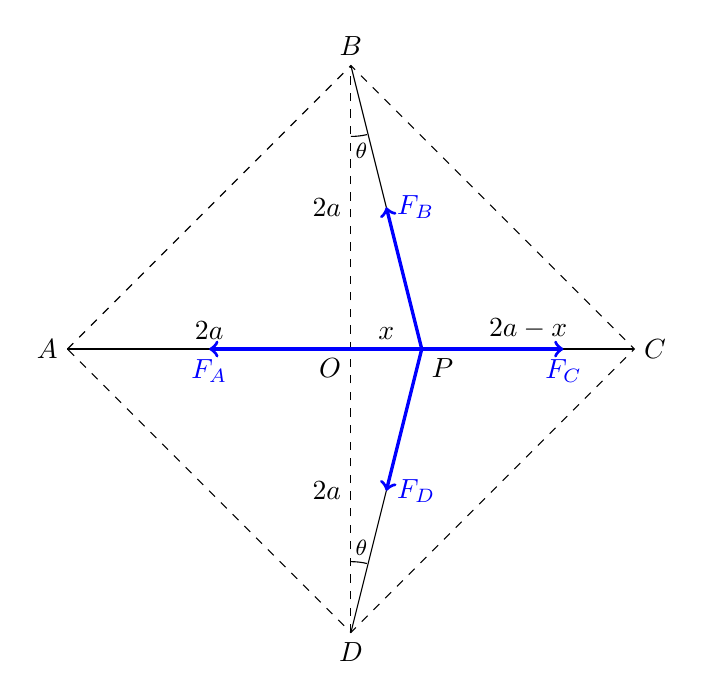
\begin{tikzpicture}[scale=.9]
		\draw[dashed] (-4,0) node[left]{$A$} -- (0,4) node[above]{$B$} -- (4,0) node[right]{$C$} -- (0,-4) node[below]{$D$} -- cycle;
		\draw (-4,0) -- (0,0) node[below left]{$O$} node[midway,above] {$2a$} -- (1,0) node[below right]{$P$} node[midway,above]{$x$} -- (4,0) node[midway,above]{$2a-x$};
		\draw (0,4) -- (1,0) -- (0,-4);
		\draw[dashed] (0,-4) -- (0,0) node[midway,left]{$2a$} -- (0,4) node[midway,left]{$2a$};
		\draw[very thick,blue,->] (1,0) -- ++(-3,0) node[below]{$F_A$};
		\draw[very thick,blue,->] (1,0) -- ++(2,0) node[below]{$F_C$};
		\draw[very thick,blue,->] (1,0) -- ++(-0.5,2) node[right]{$F_B$};
		\draw[very thick,blue,->] (1,0) -- ++(-0.5,-2) node[right]{$F_D$};
		\draw (0,3) arc(-90:-76.96:1);
		\node at (0.15,2.8) {{\footnotesize $\theta$}};
		\draw (0,-3) arc(90:76.96:1);
		\node at (0.15,-2.8) {{\footnotesize $\theta$}};
		\end{tikzpicture}
		
		Example \ref{ex-fourstrings}
	\end{minipage}\hfil
	\begin{minipage}{0.4\textwidth}
		\centering
		\begin{tikzpicture}[yscale=.9]
		\draw[fill] (0,0) node[above right]{$O$} -- (0,-5) node[right]{$N$} node[left,midway]{$a$} -- (0,-6.67) node[right]{$E$} node[left,midway]{$\frac{1}{3}a$} -- (0,-7.5) circle(0.1) node[right]{$P$} node[left,midway]{$x$};
		\draw[dashed] (0.8,-5) --++ (0.8,0) node[right,align=center,execute at begin node=\setlength{\baselineskip}{1.2em}]{{\footnotesize natural}\\ {\footnotesize position}};
		\draw[dashed] (-0.9,-6.67) --++ (0.5,0) (0.8,-6.67) --++ (0.8,0) node[right,align=center,execute at begin node=\setlength{\baselineskip}{1.2em}]{{\footnotesize equilibrium}\\ {\footnotesize position}};
		\draw[dashed] (-0.9,-7.5) --++ (0.5,0);
		\draw (-0.5,0) -- (0.5,0);
		\draw[->] (-1.2,-5) -- (-1.2,-6.67) node[left]{$0$} -- (-1.2,-7.5) node[left]{$x$} -- (-1.2,-8) node[below]{$+$};
		\draw (-1.2,-6.67) --++ (0.1,0) (-1.2,-7.5) --++ (0.1,0);
		\end{tikzpicture}
		
		Example \ref{ex-elabounce}
	\end{minipage}
\end{figure}

magnitude of resultant of $F_A$ and $F_C$ is:

{
	
	\centering
	
	$F_{AC} = F_A - F_C = \frac{\lambda}{a}(2a+x-a) - \frac{\lambda}{a}(2a-x-a) = \frac{2\lambda}{a}x$
	
}

magnitude of resultant of $F_B$ and $F_D$ is:

{
	
	\centering
	
	$F_{BD} = F_B\sin\theta + F_D\sin\theta = 2\cdot\frac{\lambda}{a}\left(\sqrt{(2a)^2+x^2} - a\right)\cdot \frac{x}{\sqrt{(2a)^2+x^2}}$
	
	\vspace*{0.1\baselineskip}
	
	$F_{BD} = \frac{2\lambda x}{a} \left(1 - \frac{a}{\sqrt{4a^2+x^2}}\right) =  \frac{2\lambda x}{a} \left\{1 - \frac{1}{2} \cdot \left(1 + \frac{x^2}{4a^2}\right)^{-\sfrac{1}{2}} \right\} $
	
}

recall binomial expansion approximation $(1+\delta)^n \approx 1 + n\delta$ for $\delta \ll 1$

given that $x \ll a$, i.e., $\frac{x}{a} \ll 1$, so one has: $\left(1 + \frac{x^2}{4a^2}\right)^{-\sfrac{1}{2}} \approx 1 -\frac{1}{2}\cdot \frac{x^2}{4a^2} $

neglecting higher powers of $\frac{x}{a}$, we find

{
	
	\centering
	
	$F_{BD} \approx \frac{2\lambda x}{a} \left(1 - \frac{1}{2} \cdot 1\right)  \RA F_{BD} \approx \frac{\lambda}{a}x$
	
}

now consider the resultant force, also note that both $F_{AC}$ and $F_{BD}$ act to the left, so

{
	
	\centering
	
	$F_\text{net} = -F_{AC} - F_{BD} \RA m\ddot{x} = -\frac{2\lambda}{a}x - \frac{\lambda}{a}x \RA \ddot{x} = -\frac{3\lambda}{ma}x $
	
}

hence particle $P$ describes simple harmonic oscillation with period $T=\frac{2\pi}{\omega} = 2\pi\sqrt{\frac{ma}{3\lambda}}$ \eoe


\example{A particle of mass $m$ is suspended at the end of an elastic cord of natural length $a$ and modulus of elasticity $3mg$. The particle is released from rest from $\frac{1}{4}a$ above the equilibrium position. (a) Show that the particle will perform simple harmonic motion. (b) Find the greatest speed during the oscillation. (c) Find when the particle first reach this maximum speed.} \label{ex-elabounce}

equilibrium when $mg=\frac{\lambda}{a}\Delta l =\frac{3mg}{a}\Delta l \RA \Delta l = \frac{1}{3}a$

so equilibrium position $E$ at $\frac{1}{3}a$ below natural position

take positive direction as vertically downwards

when particle is displaced by $x$: $F_\text{net}=mg-T = mg - \frac{\lambda}{a}\Delta l$

{
\centering

$m\ddot{x} = mg - \frac{3mg}{a} \left(\frac{1}{3}a+x\right) \RA \ddot{x} = - \frac{3g}{a}x$

}

so simple harmonics with angular frequency $\omega =\sqrt{ \frac{3g}{a}}$

at $t=0$, initial position $x(0)=-\frac{1}{4}a$, amplitude is magnitude of initial displacement $x_0 = \frac{1}{4}a$

maximum speed $v_\tmax = \omega x_0 = \sqrt{ \frac{3g}{a}} \cdot \frac{1}{4}a \RA v_\tmax = \frac{\sqrt{3ga}}{4}$

at $t=0$, $v(0)=0$, particle starts to move downwards (positive direction)

so can write down velocity-time relation: $v(t) = v_\tmax \sin \omega t$

greatest speed when $\sin\omega t=1$, or $\omega t = \frac{\pi}{2} \RA t= \frac{\pi}{2}\sqrt{\frac{a}{3g}}$ 

alternatively, note that speed becomes maximum when particle passes equilibrium position

this completes one quarter of a full oscillation, which takes $\frac{1}{4}$ of one period

so time taken to reach $v_\tmax$ is: $t=\frac{1}{4}T = \frac{1}{4}\cdot\frac{2\pi}{\omega} \RA  t=\frac{\pi}{2}\sqrt{\frac{a}{3g}}$  \eoe

\example{Consider the same oscillatory system in Example \ref{ex-elabounce}. If the particle is brought to a position where the length of the elastic string is $2a$ and released from rest. Find the distance $OP$ when particle $P$ reaches the greatest height, and also find the time taken for $P$ first comes to this height.}

when string remains taut, $P$ performs simple harmonic motion

we have found equilibrium is at $\frac{1}{3}a$ below natural position, and angular frequency $\omega=\sqrt{\frac{3g}{a}}$

amplitude of this oscillation: $x_0 = 2a - a -\frac{1}{3}a \RA x_0 = \frac{2}{3}a$

at $t=0$, initial displacement $x(0)=+x_0$, so displacement-time relation is: $x=x_0\cos\omega t$

when string becomes slack, string is at natural length, $x=-\frac{1}{3}a$, so

{

\centering

$v^2 = \omega^2 (x_0^2 - x^2) \RA v^2 = \frac{3g}{a} \left( \frac{4}{9}a^2 - \frac{1}{9}a^2 \right) \RA v=\sqrt{ga}$

$-\frac{1}{3}a = \frac{2}{3}a\cos\omega t_1 \RA \omega t_1 = \frac{2\pi}{3} \RA t_1 = \frac{2\pi}{3}\sqrt{\frac{a}{3g}}$

}

afterwards, no tension acts, $P$ is acted by gravity only, so constant acceleration of free fall

instantaneous speed becomes zero at highest point, so we have:

{

\centering

$0^2 - v^2 = 2\cdot(-g) \cdot \Delta h \RA \Delta h = \frac{v^2}{2g} = \frac{ga}{2g} \RA \Delta h = \frac{1}{2}a$

$0 - v = (-g)\cdot t_2 \RA t_2 = \frac{v}{g} = \frac{\sqrt{ga}}{g} \RA t_2 = \sqrt{\frac{a}{g}}$

}

hence greatest height is $\frac{1}{2}a$ above natural position of the string $\RA OP=a-\frac{1}{2}a=\frac{1}{2}a$

alternatively, one can also consider energy changes: elastic P.E. in string = G.P.E. gain

{

\centering

$\frac{1}{2}\cdot\frac{3mg}{a}\cdot(2a-a)^2 = mg\Delta H \RA \Delta H = \frac{3}{2}a$

}

this shows the greatest height is $\frac{3}{2}a$ above the point of release $\RA OP=2a-\frac{3}{2}a = \frac{1}{2}a$

total time taken $t=t_1+t_2 = \frac{2\pi}{3}\sqrt{\frac{a}{3g}} + \sqrt{\frac{a}{g}} \RA t = \left(\frac{2\pi}{3\sqrt{3}} + 1\right)\sqrt{\frac{a}{g}}$ \eoe

